\documentclass{article}
\usepackage{graphicx}
\usepackage{wrapfig}
\usepackage{url}
\usepackage{hyperref}
\usepackage{subcaption}
\usepackage{array}
\usepackage{caption}
\usepackage{geometry}
\geometry{margin=2.5cm}
\usepackage[francais]{babel}

\title{Projet de recherche documentaire\\ \large Génération procédurale de décors}
\author{Killian Mathias\\ Matthéo Girardclos}
\date{January 2025}

\begin{document}

\maketitle
\tableofcontents
\newpage
\section{Introduction}

En informatique, la génération procédurale fait référence à la création automatique de contenu numérique, que ce soit des éléments en 2D ou 3D, des scénarios, des dialogues, ou même des niveaux de jeu. Cette technique s'appuie sur des algorithmes qui permettent de produire une grande quantité de contenu sans nécessiter l'intervention directe d'un humain. Elle est particulièrement prisée dans les secteurs du jeu vidéo et du cinéma, où elle aide à créer des environnements variés et immersifs.  Un exemple marquant de cette méthode est le jeu Minecraft, qui génère un monde ouvert de manière procédurale grâce à différentes couches d'algorithmes. D'autres jeux, comme Terraria ou No Man’s Sky, utilisent également cette approche pour offrir des mondes dynamiques et uniques.\par
Créer des décors qui soient à la fois aléatoires et cohérents représente un vrai défi. Par exemple, modéliser des reliefs comme des montagnes ou des plaines peut être assez complexe. La génération procédurale aide à surmonter ce problème en appliquant des algorithmes adaptés, ce qui évite de devoir concevoir chaque carte de jeu à la main.\par
  Dans le cadre de ce projet, notre but est de développer une version simplifiée de Terraria, un jeu de survie en 2D. Ce jeu, jouable en solo ou en multijoueur, permet aux joueurs d'explorer un monde divisé en biomes, de récolter des ressources et d'interagir avec leur environnement. Nous allons nous concentrer sur la génération du monde, des biomes et éventuellement des grottes, tout en veillant à optimiser l'implémentation pour garantir de bonnes performances.


\section{Différentes approches}

Afin de générer procéduralement un décor il existe plusieurs approches. Tout d'abord, les objectifs d'une implémentation à une autre ne sont pas exactement les mêmes, cependant cela reste de la génération procédurale. Dans cette section, nous présenterons plusieurs méthodes populaires, en les analysant sous l’angle de leur efficacité et de leur applicabilité à notre projet de génération d’un monde 2D de type Terraria.\par

Tout d'abord afin de répondre à nos besoins nous devons créer des paysages avec des reliefs réalistes.

\subsection{Génération de terrains et de reliefs}

Pour créer des paysages avec des reliefs il existe deux algorithmes qui sont respectivement le bruit de Perlin et le bruit Simplex.

D'après la page Wikipédia \cite{perlin}, le bruit de Perlin, développé par Ken Perlin en 1985, est un système de génération pseudo-aléatoire. Ce dernier cherchait à éliminer le look "machinique" des effets spéciaux du film \textit{TRON.} Son utilité principale est la génération procédurale de décors au nombre de dimensions que l'on souhaite mais il est plus fréquemment utilisé à 2 ou 3 dimensions. Nous rentrerons dans les détails de cet algorithme plus tard.\par
Le bruit Simplex \cite{simplex_noise} a également été créé par Ken Perlin en 2001 avec le but de remédier aux limites de son algorithme précédent. Il est assez similaire au bruit de Perlin, mais il est plus efficace et est généralement utilisé pour travailler avec des espaces à plus de 3 dimensions. Nous ne verrons pas en détail cet algorithme, car bien qu'il soit plus performant, il est moins documenté que son prédécesseur et donc logiquement plus difficile à comprendre.
\begin{wrapfigure}{r}{0.25\textwidth} % 'r' pour droite, largeur ajustée
  \centering
  
\includegraphics[width=0.22\textwidth]{assets/Perlin_noise.jpg}
  \caption{Bruit de Perlin à 2 dimensions}
  \label{perlin}
\end{wrapfigure}

\subsection{Génération de biomes}

Après la génération de nos terrains, nous prévoyons d'implémenter un système de biomes. Chaque biome, représentant une zone particulière du terrain, aura ses propres caractéristiques visuelles, avec des blocs dont les textures varieront selon le biome où ils se trouvent. Pour ce faire, il existe deux approches qui sont respectivement le Bruit Worley (ou Voronoï) et définir une carte avec des températures et une humidité.\par
La première approche a été créée par Steven Worley en 1996, et possède trois noms : le Bruit de Worley \cite{worley_noise}, le bruit de Voronoï et le bruit Cellulaire. Cette approche se base sur le diagramme de Voronoï \cite{voronoi_diagram}, qui est un découpage d'un plan sous forme de cellules. Dans notre cas, cette méthode n'est pas forcément pertinente car elle est plus efficace sur un plan plutôt qu'en deux dimensions comme nous et les transitions entre les biomes seraient trop brutales.\par
La seconde approche serait donc optimale car on pourrait réutiliser les algorithmes pour la génération de terrains directement pour les biomes. En effet, le Bruit de Perlin, en plus de générer les terrains, peut également nous permettre de définir une humidité ainsi qu'une température pour chaque bloc, ce qui nous permettra d'avoir de meilleures transitions entre les biomes et permettre une expérience plus agréable au joueur. On s'orientera donc vers cette approche-là car elle correspond plus à nos besoins. 

\subsection{Génération de grottes et de cavernes}
Une fois notre terrain et nos biomes générés, afin de notre implémentation se rapproche le plus de Terraria, il faut générer des cavernes et des grottes souterraines. Il existe également deux approches différentes pour concevoir cela qui sont le Random Walk \cite{random_walk} (ou Marche Aléatoire) et une méthode qui utilise des automates cellulaires \cite{automate_cellulaire}.\par
La première méthode est un modèle mathématique qui permet de créer des donjons ainsi que des réseaux de tunnels. Nous nous focaliserons pas sur cette méthode car elle n'est pas utilisée par Terraria et que cela s'éloigne de la génération procédurale.\par 
La seconde méthode, utilisée par Terraria mais également par le jeu de la vie, consiste en une grille régulière de cellule, et une cellule évolue en fonction de ses voisines ce qui permet de générer des grottes réalistes.

\subsection{Génération de minerais et ressources}
Maintenant que les grottes sont générées, il faudrait que le joueur puisse récolter des ressources. Nous n'irons pas aussi loin dans l'implémentation cependant nous générerons quand même des minerais. Il existe différentes méthodes qui permettent cela et qui sont la distribution par couches (ou Stratification \cite{stratification}) et le Bruit de Perlin appliqué au minerais. \par
La première méthode est utilisée par Minecraft en combinaison avec le Bruit de Perlin, la seconde se combine avec la génération de terrain et donc nous utiliserons cette méthode car c'est également celle utilisée par Terraria. Nous verrons plus en détail comment nous l'utiliserons pour notre implémentation à la section \ref{Implémentation}.


\subsection{Comparaison et choix des méthodes pour notre projet}

Comme nous avons pu le préciser lors des paragraphes précédents, la méthode de génération procédurale que nous utiliserons est le Bruit de Perlin car elle bien bien documentée et cela nous facilitera pour notre implémentation. De plus cette méthode nous sera également utile pour générer des biomes et des minerais, ce qui réduira de manière conséquente le travail réalisé. Enfin, pour générer nos grottes nous nous orienterons vers la méthode qui utilise les automates cellulaires car c'est la méthode utilisée par Terraria, cela nous paraît donc évident d'utiliser la même méthode. 

\section{Méthodologie}

Nous avons vu ci-dessus les différents moyens d'appliquer la génération procédurale et les applications liées à ces moyens. Maintenant, nous devons définir une méthodologie afin de réaliser notre implémentation à partir des recherches effectuées.

\subsection{Les outils utilisés}
Afin de nous concentrer un maximum sur la recherche et l'application directe de la génération procédurale, nous avons choisi un langage que nous maîtrisons bien mais qui est bien documenté, Python. De plus, si nous voulons réaliser un jeu vidéo, nous ne pouvons pas le faire nativement et simplement, c'est pour cela que nous avons choisi le module Pygame, qui offre simplicité mais aussi une très bonne documentation, ce qui facilite l’appréhension de ce dernier.\par
\begin{figure}[!h]
  \centering
  \begin{subfigure}[b]{0.2\textwidth}
    \centering
    
\includegraphics[width=\textwidth]{assets/python_logo.png}
    \caption{Logo Python}
  \end{subfigure}
  \hspace{0.6cm}
  \begin{subfigure}[b]{0.2\textwidth}
    \centering
    
\includegraphics[width=\textwidth]{assets/pygame_logo.png}
    \caption{Logo Pygame}
  \end{subfigure}
  \caption{Logos des bibliothèques Python et Pygame}
  \label{fig:logos_python}
  
\end{figure}
Comme dit précédemment, nous connaissions déjà le langage python, nous n'avons donc pas eu beaucoup à apprendre. Cependant, le module Pygame était tout nouveau pour nous, nous nous sommes donc aidés de la documentation, de tutoriels sur YouTube mais aussi d'un livre \cite{prieur2019pygame}.\par

Puisque ce projet devait se réaliser en duo, il nous fallait à tout prix un outil pour travailler et collaborer. Dans un premier temps, pour la communication nous avons utilisé Discord, qui est très pratique car on peut échanger via des messages, des appels audios, vidéos mais cet outil offre également la possibilité de partager son écran directement en appel. Le second outil de collaboration utilisé est Git avec Github afin de partager le code. C'est actuellement sur le marché le meilleur outil de versioning et de collaboration. De plus, afin d'adopter une méthode agile et travailler sans se répeter, nous avons utilisés l'outil Jira. Il permet de créer des tickets qui correspondent à des tâches à effectués, puis de définir des périodes de Sprint, période où l'on effectue un ensemble de tickets.\cite{cochoy2011perlin}

\begin{figure}[!h]
  \centering
  \begin{subfigure}[b]{0.2\textwidth}
    \centering
    
\includegraphics[width=0.5\textwidth]{assets/discord.png}
    \caption{Logo Discord}
  \end{subfigure}
  \hspace{0.6cm}
  \begin{subfigure}[b]{0.2\textwidth}
    \centering
    
\includegraphics[width=0.6\textwidth]{assets/git.png}
    \caption{Logo Git}
  \end{subfigure}
  \hspace{0.6cm}
  \begin{subfigure}[b]{0.2\textwidth}
    \centering
    
\includegraphics[width=\textwidth]{assets/jira.png}
    \caption{Logo Jira}
  \end{subfigure}
  \caption{Logos des outils de communication et de collaboration}
  \label{fig:logos_collab}
  
\end{figure}

\subsection{Organisation du code}
Pour avoir un code propre, et pour faciliter la compréhension entre nous, nous avons décidé au préalable d'une organisation et d'une structure de base. Le but était de créer un squelette de code qui nous permettrait de nous y retrouver facilement. Nous avons donc décidé de créer plusieurs fichiers, un pour chaque classe implémentée, chacun ayant une fonction précise. Nous avons pour cela créé un diagramme UML de classes que nous pouvons voir à la figure \ref{UML_class}.\par
Nous avons tout d'abord une classe Tile qui hérite de pygame.Sprite du module Pygame car elle propose des méthodes pour gérer les collisions de manière optimale avec les tuiles, et ses sous classes qui sont les différents types de blocs que l'on peut trouver dans le jeu. Ces blocs seront générés un à un procéduralement et seront destructibles, d'où l'utilité des les définir un à un.\par
Ensuite, nous avons la classe World qui va être la classe responsable de la génération du monde de manière procédurale. Elle va notamment avoir pour attribut une matrice de Tuiles car notre jeu est dans un espace à deux dimensions.\par
Puis, nous avons la classe Player qui va gérer le joueur, ses déplacements, ses interactions avec le monde et les blocs. Cette classe va hériter de classe pygame.Sprite.\par
Enfin, la classe Game qui va être la classe principale du jeu, elle va gérer la boucle principale du jeu, les événements, l'affichage et le rafraîchissement de l'écran.\par
\begin{figure}[!h]
  \centering
  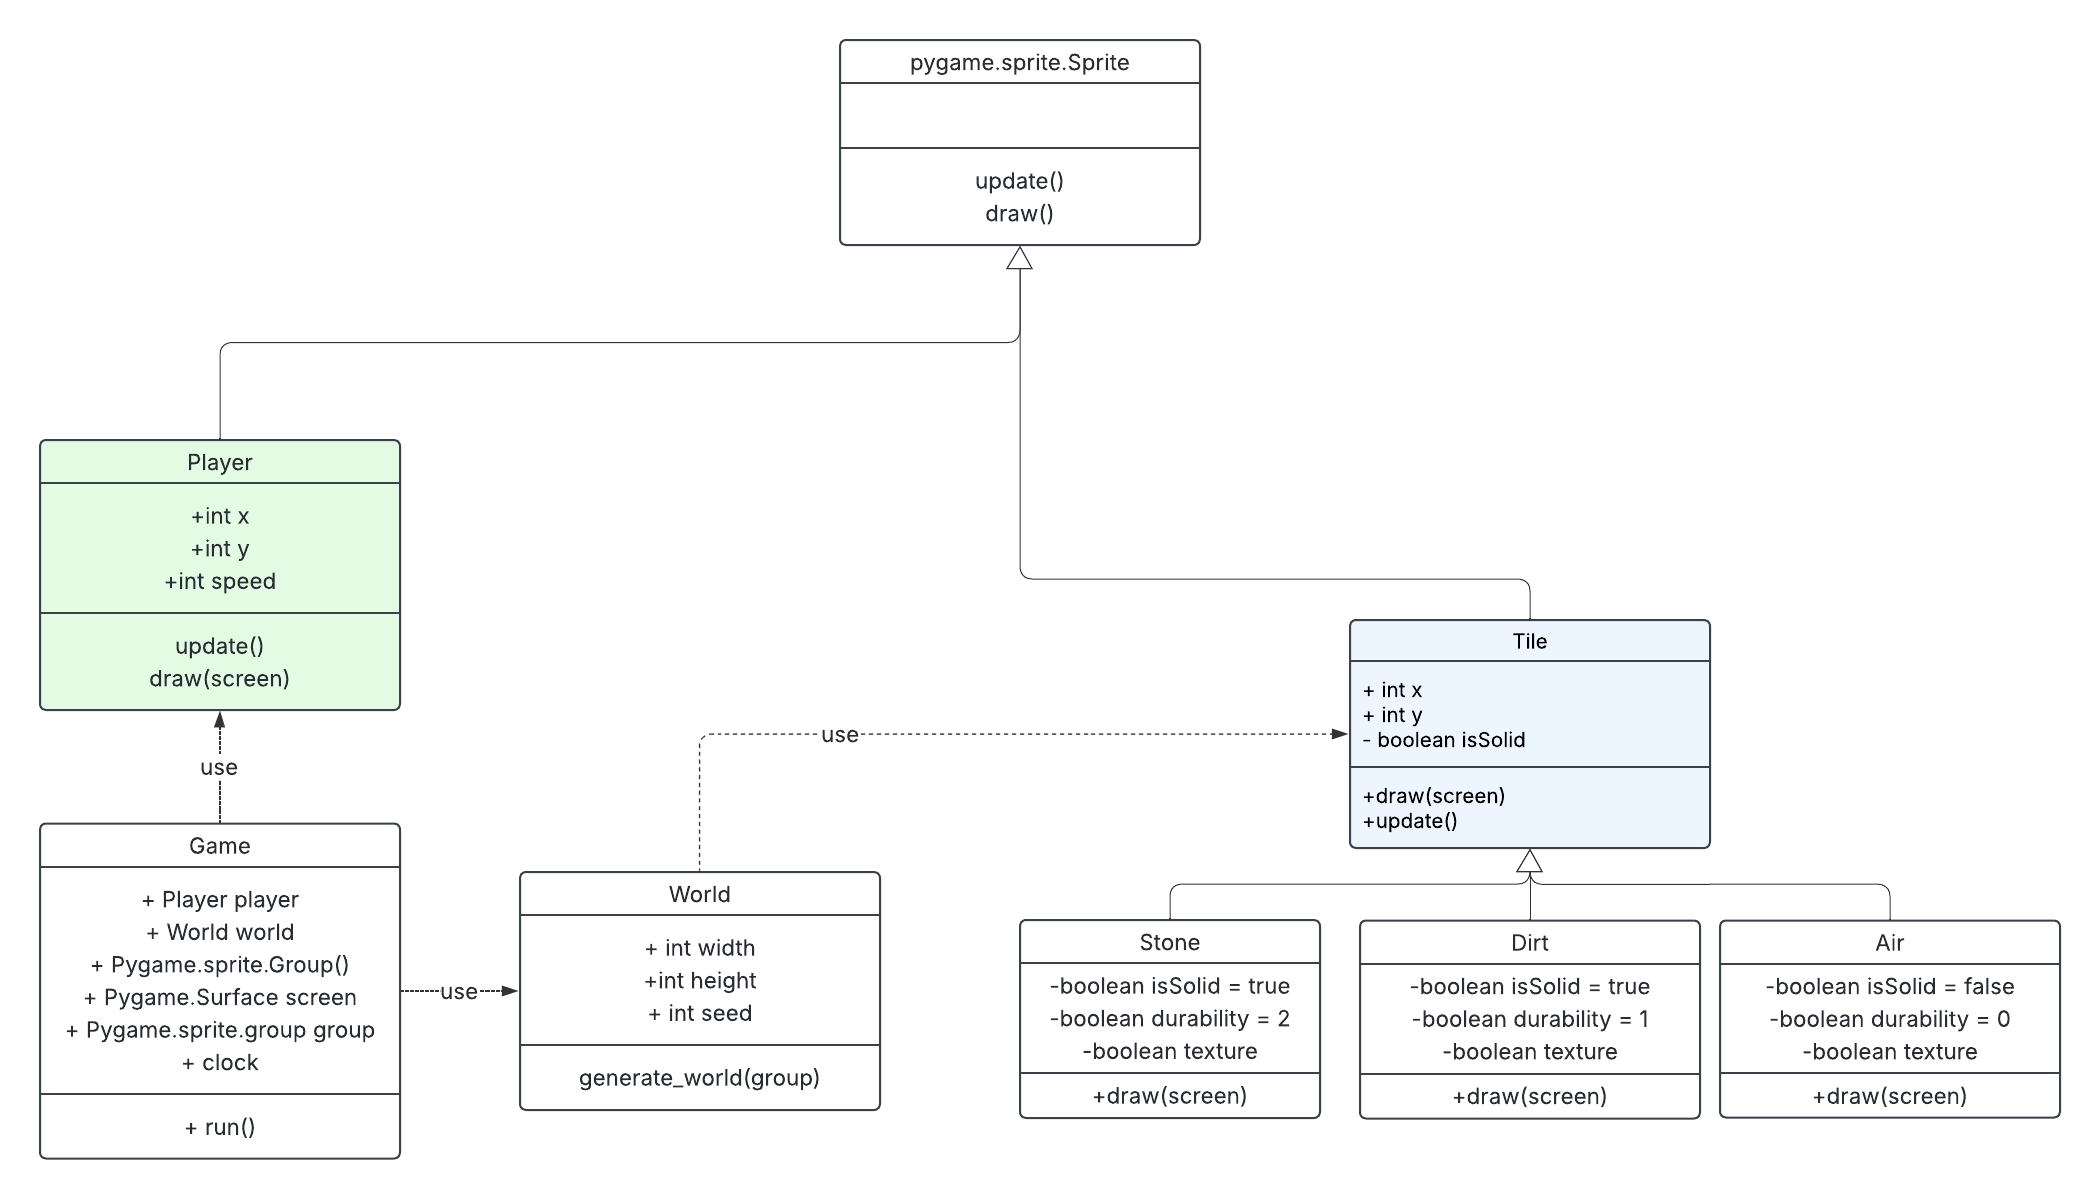
\includegraphics[width=\textwidth]{assets/UML_class.png}
  \caption{Diagramme de classe du Terraria-Like}
  \label{UML_class}
\end{figure}

Maintenant que nous avons définit comment nous allions aborder ce projet ambitieux, nous allons voir comment nous avons implémenté notre reproduction de Terraria.
\section{Implémentation et Résultats}
\label{Implémentation}

Avant même de commencer à avoir un terrain qui se génère procéduralement, il a déjà fallut instaurer les bases de notre implémentation.

\subsection{Bases du jeu}
  Tout d'abord, nous avons dû créer une fenêtre de jeu avec Pygame, puis définir la taille de la fenêtre. Ensuite, nous avons dû créer une boucle principale qui va gérer les événements du jeu, l'affichage et le rafraîchissement de l'écran avec trois méthodes qui sont respectivement \textbf{handling\_events}, \textbf{display} et \textbf{update}. Nous avons également dû définir un nombre de FPS (Images par secondes) afin d'avoir un affichage fluide et pas trop exigeant en ressources.\par
Une fois l'étape précédente réalisé, nous avons implémenté le joueur grâce à la classe Player. Ce dernier est défini par une boîte de collision, nommée \textbf{rect}, et une texture. Il peut se déplacer dans les quatre directions bien que le déplacement vers le bas corresponde à la gravité et le déplacement vers le haut à un saut.\par
\subsection{Génération procédurale du terrain}
La base de notre jeu est maintenant instaurée, avec un personnage qui peut se déplacer dans la fenêtre. Cependant, nous n'avons pas encore de décor, ni de monde. C'est ici que va intervenir la génération procédurale.\par
Afin de bien comprendre comment nous nous y sommes pris dans un premier temps pour générer un terrain avec du relief, nous allons expliquer le fonctionnement du Bruit de Perlin à une dimension. Tout d'abord, nous avons définit un tableau de valeurs aléatoires entre -1 et 1.\par
\begin{table}[h]
  \centering
  \begin{tabular}{|c|c|c|c|c|}
  \hline
  0.42 & -0.87 & 0.15 & -0.33 & 0.98\\
  \hline
  \end{tabular}
  \caption{Exemple de tableau de valeurs aléatoires avec x égal à 5}
  \label{tableau_aleatoire}
  \end{table}
  Une fois que nous avons obtenu notre tableau de valeurs, nous allons le lisser plusieurs fois à l’aide d’un algorithme. L’objectif est que, après avoir multiplié ces valeurs par une hauteur maximale (appelée valeur de y maximum), la différence entre deux valeurs voisines soit au maximum de 1. Cela permet d’obtenir une transition douce et progressive entre les valeurs, sans saut brusque. Ce processus va donc nous permettre d'avoir un terrain avec du relief réaliste. Dans un premier temps, on choisit que la tuile la plus haute sur chaque colonne est un bloc d'herbe et les tuiles en dessous de la Terre. Par défaut, le reste des tuiles sont de l'air.\par
\subsection{Collisions}
  Notre terrain est maintenant opérationnel et le joueur peut donc se déplacer dessus à une exception près, les collisions. En effet, bien que notre personnage puisse se déplacer, il peut passer à travers le terrain et les tuiles générées. Comme le joueur, les tuiles sont aussi définies par un \textbf{rect}. Nous avons donc utilisé la méthode \textbf{collide\_rect} de Pygame qui va détecter les collisions entre le joueur et les tuiles (sauf les tuiles de type air) grâce à leurs \textbf{rect}. Ensuite, il suffit juste de dire que le joueur ne peut pas se déplacer dans la direction de la collision et notre personnage pourra se mouvoir sur le terrain sans passer à travers. \par

  \subsection{Génération procédurale des biomes}
\section{Conclusion et Perspectives}

\section{Bibliographie et références}
\bibliographystyle{alpha}
\bibliography{bibliography}

\end{document}
